\documentclass[border=4pt]{standalone}
\usepackage{fontspec}
\usepackage{amsmath}
\usepackage{unicode-math}
\setmainfont{Latin Modern Roman}
\setmathfont{Latin Modern Math}
\usepackage{pgfplots}
\usepackage{pgfplotstable}
\pgfplotsset{compat=1.18}
\usepackage{tkz-euclide}
\usetikzlibrary{arrows.meta,calc,angles,quotes,patterns,3d,backgrounds}
\definecolor{ink}{HTML}{123428}
\definecolor{asy}{HTML}{475569}
\definecolor{mint}{HTML}{86e0bd}
\tikzset{asym/.style={asy, line width=0.9pt, dash pattern=on 5pt off 3.5pt},
         guide/.style={gray!70, line width=0.6pt, densely dotted},
         dot/.style={circle, inner sep=0pt, minimum size=5pt, draw=white, line width=0.5pt},
         odot/.style={circle, inner sep=0pt, minimum size=5.5pt, fill=white, line width=1pt},
         lab/.style={font=\footnotesize, inner sep=1.5pt, text=ink}}
\begin{document}
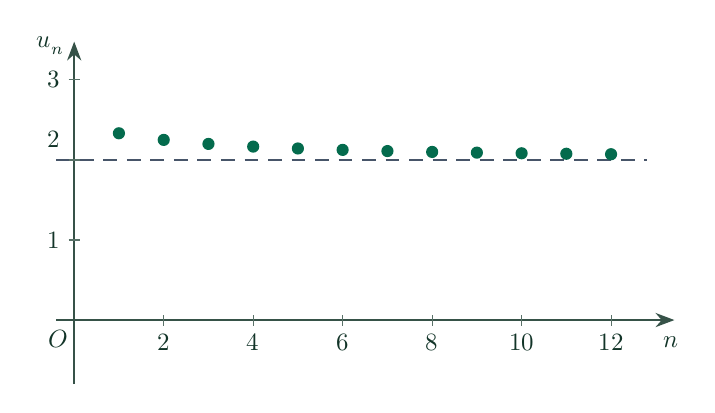
\begin{tikzpicture}
\draw[ink!85, line width=0.7pt, -{Stealth[length=2.4mm]}] (0.000,0.814) -- (7.850,0.814);
\draw[ink!85, line width=0.7pt, -{Stealth[length=2.4mm]}] (0.227,0.000) -- (0.227,4.350);
\draw[asy, line width=0.8pt, dash pattern=on 5pt off 3.5pt] (0.000,2.847) -- (7.500,2.847);
\fill[color={rgb,255:red,4;green,107;blue,77}] (0.795,3.186) circle (2.2pt);
\fill[color={rgb,255:red,4;green,107;blue,77}] (1.364,3.102) circle (2.2pt);
\fill[color={rgb,255:red,4;green,107;blue,77}] (1.932,3.051) circle (2.2pt);
\fill[color={rgb,255:red,4;green,107;blue,77}] (2.500,3.017) circle (2.2pt);
\fill[color={rgb,255:red,4;green,107;blue,77}] (3.068,2.993) circle (2.2pt);
\fill[color={rgb,255:red,4;green,107;blue,77}] (3.636,2.975) circle (2.2pt);
\fill[color={rgb,255:red,4;green,107;blue,77}] (4.205,2.960) circle (2.2pt);
\fill[color={rgb,255:red,4;green,107;blue,77}] (4.773,2.949) circle (2.2pt);
\fill[color={rgb,255:red,4;green,107;blue,77}] (5.341,2.940) circle (2.2pt);
\fill[color={rgb,255:red,4;green,107;blue,77}] (5.909,2.932) circle (2.2pt);
\fill[color={rgb,255:red,4;green,107;blue,77}] (6.477,2.926) circle (2.2pt);
\fill[color={rgb,255:red,4;green,107;blue,77}] (7.045,2.920) circle (2.2pt);
\draw[ink!70] (1.364,0.744) -- (1.364,0.884);
\draw[ink!70] (2.500,0.744) -- (2.500,0.884);
\draw[ink!70] (3.636,0.744) -- (3.636,0.884);
\draw[ink!70] (4.773,0.744) -- (4.773,0.884);
\draw[ink!70] (5.909,0.744) -- (5.909,0.884);
\draw[ink!70] (7.045,0.744) -- (7.045,0.884);
\draw[ink!70] (0.157,1.831) -- (0.297,1.831);
\draw[ink!70] (0.157,2.847) -- (0.297,2.847);
\draw[ink!70] (0.157,3.864) -- (0.297,3.864);
\node[font=\small, text=ink] at (7.800,0.534) {$n$};
\node[font=\small, text=ink] at (-0.073,4.300) {$u_n$};
\node[font=\small, text=ink, inner sep=0.5pt, fill=white] at (1.364,0.534) {$2$};
\node[font=\small, text=ink, inner sep=0.5pt, fill=white] at (2.500,0.534) {$4$};
\node[font=\small, text=ink, inner sep=0.5pt, fill=white] at (3.636,0.534) {$6$};
\node[font=\small, text=ink, inner sep=0.5pt, fill=white] at (4.773,0.534) {$8$};
\node[font=\small, text=ink, inner sep=0.5pt, fill=white] at (5.909,0.534) {$10$};
\node[font=\small, text=ink, inner sep=0.5pt, fill=white] at (7.045,0.534) {$12$};
\node[font=\small, text=ink, inner sep=0.5pt, fill=white] at (-0.028,1.831) {$1$};
\node[font=\small, text=ink, inner sep=0.5pt, fill=white] at (-0.028,3.107) {$2$};
\node[font=\small, text=ink, inner sep=0.5pt, fill=white] at (-0.028,3.864) {$3$};
\node[font=\small, text=ink, inner sep=0.5pt] at (0.027,0.574) {$O$};
\end{tikzpicture}
\end{document}
